\documentclass[a4paper]{article}
\usepackage[a4paper, left=1.8cm, right=1.8cm, top=2.5cm, bottom=2.5cm]{geometry}
\usepackage{ctex}
\usepackage{amsmath}
\usepackage{makecell}
\usepackage{xcolor}
\usepackage{listings}
\usepackage{hyperref}
\usepackage{url}
\usepackage{float}

\usepackage{graphicx}
\usepackage{caption}

\lstset{
    language = [x86masm]Assembler,
    xleftmargin = 3em,xrightmargin = 3em, aboveskip = 1em,
	backgroundcolor = \color{white}, % 背景色
	basicstyle = \normalsize\ttfamily, % 基本样式 + 小号字体
	rulesepcolor= \color{gray}, % 代码块边框颜色
	breaklines = true, % 代码过长则换行
	numbers = left, % 行号在左侧显示
	numberstyle = \footnotesize, % 行号字体
    numbersep = 14pt, 
	keywordstyle = \color{blue!50!red!100}, % 关键字颜色
	commentstyle =\color{red!50!green!50!blue!60}, % 注释颜色
	stringstyle = \color{red}, % 字符串颜色
	frame = none, % 用(带影子效果)方框框住代码块
	showspaces = false, % 不显示空格
	columns = fixed, % 字间距固定
} 

\begin{document}
\begin{center}
    {{\zihao{3} \heiti 编译原理实践项目报告}}
\end{center}
~\\[-3em]
\begin{center}
    \zihao{4}
    \begin{tabular}{>{\raggedleft}m{3em} >{\centering\arraybackslash}m{7em}}
    学号: & 10225101460 \\[-3ex] % 控制行距
     & \hrulefill \\[-1ex]
    姓名: & 李鹏达 \\[-3ex]
    & \hrulefill \\
    \end{tabular}
\end{center}

\zihao{4}
\section{项目简介}

本项目主要包括正则引擎、编译器词法分析、语法分析、语义分析和中间代码生成等部分,支持自定义词法、语法和语义动作,还额外包括了``\texttt{simple\_cc}'' ——一个C语言子集的编译器,支持生成中间代码和二进制代码。项目的结构如Listing \ref{fig:struct} 所示。

\begin{lstlisting}[numbers=none,caption={项目结构},label={fig:struct}]
compiler/                   # 项目根目录
├── build/                  # 构建输出目录
├── educoder/               # 头歌平台代码
│   ├── lexer.cpp           # 词法分析实现
│   ├── LL1.cpp             # LL(1) 分析器
│   ├── semantic.cpp        # 语义分析器
│   └── SLR.cpp             # SLR 分析器
├── include/                # 头文件目录
│   ├── grammar/            # 文法接口
│   ├── lexer/              # 词法接口
│   ├── regex/              # 正则接口
│   ├── semantic/           # 语义接口
│   └── utils.hpp           # 工具函数声明
├── simple_cc/              # 编译器主程序
├── src/                    # 源文件目录
│   ├── grammar/            # 文法实现
│   ├── lexer/              # 词法实现
│   ├── regex/              # 正则实现
│   ├── semantic/           # 语义实现
│   └── utils.cpp           # 工具函数定义
├── tests/                  # 单元测试
├── .clang-format           # 格式化配置
├── .clang-tidy             # 静态检查配置
├── .gitignore              # Git 忽略配置
├── CMakeLists.txt          # CMake 构建配置
├── compile_commands.json   # 编译数据库
└── coverage.sh             # 覆盖率脚本
\end{lstlisting}

项目的仓库地址是 \url{https://github.com/llipengda/compiler}。

\section{项目亮点}

\subsection{代码量和规范写法}

本项目的代码量较大,排除重复代码后共6121行,其中3924行用于实现基础功能,1458行实现了 ``\texttt{simple\_cc}'' 的编译器功能,739行是测试代码。

代码遵循了良好的编程规范,使用 \texttt{cmake} 进行构建,使用 \texttt{clang-format} 进行代码格式化,使用 \texttt{clang-tidy} 进行代码检查,
\texttt{google-test} 进行单元测试,保证了代码的可读性和可维护性。

项目充分利用了 \texttt{C++} 的面向对象特性,使用了多态、继承和模板等特性,使得代码结构清晰,易于扩展和维护。

在实现中,所有的语法分析器都继承自\texttt{grammar\_base} 类,由其实现通用的FITRST集、 FOLLOW集的构建等功能,具体的语法分析逻辑则在子类中实现。LR(1)语法分析器继承自SLR语法分析器,仅重写构建闭包和reduce的函数,便能实现LR(1)语法分析器的功能。对于语义分析,所有的嵌入了语义分析的语法分析器继承自相应类,仅需几行代码便可实现语义分析的嵌入。这种设计使得不同的语法分析器可以共享通用的功能,同时又能根据具体的文法规则实现特定的分析逻辑。


同时,项目基于 \texttt{C++20} 标准,充分利用了现代 \texttt{C++} 的特性,如范围 for 循环、智能指针等,提升了代码的安全性和可读性。

项目充分使用模块化设计思想,将各个编译阶段的功能分离并封装为独立组件,确保系统具备良好的可扩展性与可维护性。例如,如果想使用\texttt{std::regex} 替换项目中的正则引擎,可以非常容易地实现。事实上,项目也提供了编译选项 \texttt{USE\_STD\_REGEX}来完成这一替换。

\subsection{理论课算法的自动化实现}

本项目系统地实现了编译原理课程中涉及的多项核心算法,涵盖词法分析、语法分析、语义分析及中间代码生成等关键阶段,力求将理论知识程序化、自动化,提升对编译过程整体机制的理解与掌握。

在词法分析阶段,项目基于正则表达式的直接构造法完成了从正则表达式到NFA、再到DFA的自动化转换过程。通过状态合并与跳转优化,构造出高效的有限自动机,用于识别输入文本中的词法单元(Token)。系统支持用户自定义正则表达式集合与对应的词法类别,具备良好的扩展性和实用性。同时,针对空白符、注释等可忽略符号类型,实现了灵活的过滤机制,确保词法分析器输出结果的精确性与可控性。

在语法分析方面,项目分别实现了LL(1)、SLR(1) 和 LR(1) 三种常见的自底向上与自顶向下分析算法。各算法均具备FIRST集和FOLLOW集的自动计算、分析表的构造及分析过程的模拟执行等功能。语法分析器能够自动处理用户提供的上下文无关文法,对其合法性进行检查,并在冲突可处理的前提下生成对应的分析结构。分析结果支持详细输出,便于验证算法正确性与分析流程的可视化呈现。

在语义分析阶段,项目基于属性文法模型设计并实现了语义规则的自动处理系统。支持综合属性和继承属性的定义与传播机制,可用于完成静态类型检查、符号表管理等常见语义分析任务。同时,系统集成了语法制导翻译(SDT)功能,在语法分析的过程中实时生成中间代码,为后续中间表示优化和目标代码生成打下基础。

整体系统采用模块化设计思想,将各个编译阶段的功能分离并封装为独立组件,确保系统具备良好的可扩展性与可维护性。所有模块均支持用户自定义输入(如正则表达式、文法规则、语义动作等),从而适配不同的语言子集或实验需求。同时,系统提供必要的调试与日志支持,有助于观察编译流程中各阶段的内部状态与处理结果。

\subsection{符号表存储方式}

本项目符号表采取链式符号表,为每个作用域使用哈希表维护一个符号表,并将作用域链式连接起来。当作用域结束时,自动释放该作用域内的符号,以节省内存空间。

符号表的实现充分考虑了作用域的嵌套和符号的查找效率,支持符号的插入、删除和查找操作,并支持变量遮盖。该符号表拥有 $O(1)$ 的平均插入时间复杂度和 $O(k)$ 的平均查找时间复杂度($k$ 为作用域嵌套层数,通常较小,可视为常数),同时仅有 $O(n)$ 的空间复杂度,达到了时间和空间的平衡,实现了高效的符号管理。

\subsection{错误处理}

本项目在词法分析、语法分析和语义分析阶段均实现了错误处理机制,能够检测并报告错误,并实现一定程度上的错误恢复。在语法分析和语义分析阶段,还预留了错误处理接口,允许用户自定义错误处理逻辑。

在LL(1)语法分析中,项目采用启发式错误恢复策略,通过插入、删除和替换等操作,尽量恢复到一个合法的状态,以继续分析。在LR语法分析中,项目实现了错误恢复表,能够在遇到错误时,根据当前状态和输入符号,选择合适的恢复动作。在语义分析阶段,项目为语义动作提供了错误处理接口,允许用户在语义动作中实现自定义的错误处理逻辑。

\section{额外测试}

项目使用 \texttt{google-test} 进行单元测试,覆盖了正则表达式、词法分析、语法分析、语义分析和中间代码生成等核心功能。测试用例包括正常情况和异常情况,确保各个模块的功能正确性和鲁棒性。项目测试用例共 151个,代码覆盖度达 89\%,满足了项目的质量要求。
图 \ref{fig:test} 展示了测试截图,可见151个测试用例全部通过,图 \ref{fig:coverage} 展示了测试覆盖率报告。

\begin{figure}[H]
\centering
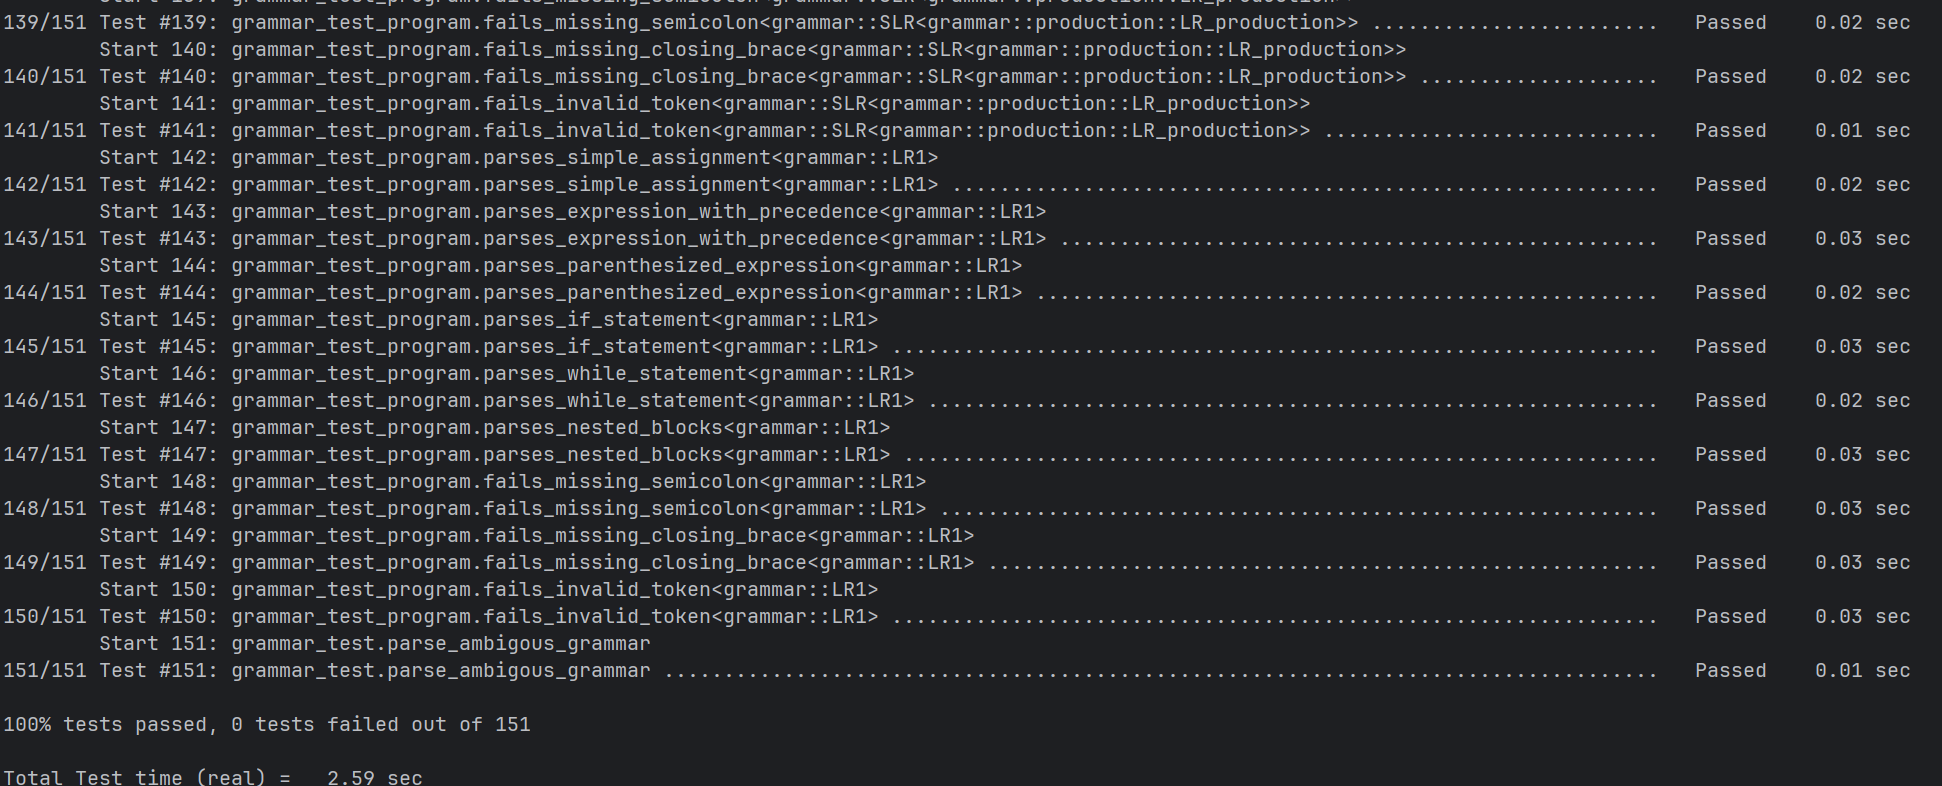
\includegraphics[width=\textwidth]{22.png}
\caption{测试截图}
\label{fig:test}
\end{figure}

\begin{figure}[H]
\centering
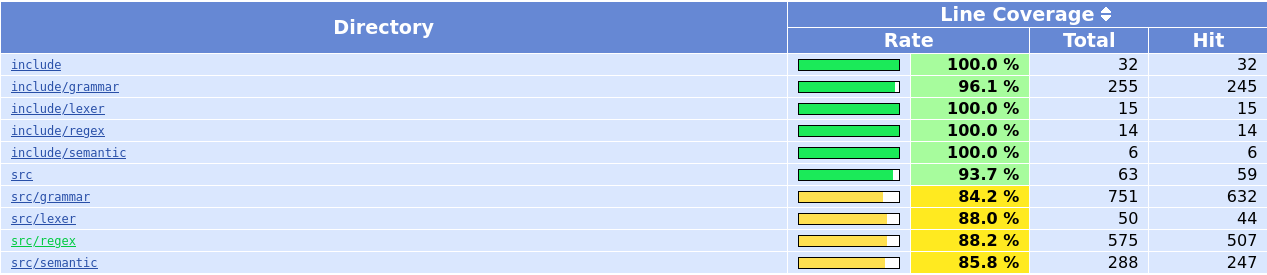
\includegraphics[width=\textwidth]{11.png}
\caption{测试覆盖率报告}
\label{fig:coverage}
\end{figure}

额外的测试保障了代码质量和泛用性,在测试过程中发现并修复了14个潜在的 bug,相助提升了代码的稳定性和可靠性。

\section{其他特色}

\subsection{正则引擎}

本项目实现了一个高效的正则引擎,支持正则表达式的直接构造法。

正则引擎能够处理常见的正则表达式语法,并支持多种匹配模式,如直接匹配和最大匹配。该正则引擎支持拓展的正则语法,如空白字符、数字、字母等,还支持字符类和字符类中的否定,可以支持如
\begin{lstlisting}[numbers=none]
(//[^\n]*)|(/\*([^*]|\*+[^*/])*\*+/)
\end{lstlisting}
这样的复杂正则表达式。

而且,该正则引擎效率较高,能够在大规模文本中快速匹配正则表达式,甚至超过 \texttt{std::regex} 的性能。

\subsection{任意文法输入的语法分析}

本项目实现了 LL(1)、SLR(1)和LR(1) 语法分析器,支持任意文法的输入。用户可以通过自定义文法规则,使用项目提供的接口进行语法分析。

\subsection{任意SDT输入的语义分析}

本项目实现了基于属性文法的语义分析器,支持任意语义动作的输入。用户可以通过自定义语义动作,使用项目提供的接口进行语义分析。

通过将语义动作嵌入产生式,并构建插入了语义动作的语法树,项目能够实现任意语义动作的执行。用户可以在语义动作中实现自定义的语义分析逻辑,如类型检查、符号表管理等。

基于这一功能,项目可以在语义分析阶段直接生成中间代码,支持用户自定义的中间代码生成逻辑。

\subsection{高扩展性}

本项目的设计充分考虑了扩展性,用户可以通过自定义正则表达式、文法规则和语义动作,轻松扩展项目的功能。同时,项目的模块化设计使得各个组件之间的耦合度较低,便于后续的维护和升级。

\subsection{高效数据结构的使用}
本项目在实现中充分利用了高效的数据结构,项目中大量使哈希表数据结构(\texttt{std::unordered\_set} 和 \texttt{std::unordered\_map}),保证了符号表、FIRST集、FOLLOW集等数据结构的高效存储和查找。同时,项目还使用了 \texttt{std::vector} 等 STL 容器,确保了数据的灵活性和高效性。

\subsection{C语言子集编译器}

本项目实现了一个C语言子集的编译器,支持基本的语法和语义分析,能够将C语言子集代码编译为中间代码和二进制代码。该编译器基于项目提供的正则引擎、词法分析器、语法分析器和语义分析器,能够处理C语言的基本语法结构,如变量声明、表达式、控制语句等。

\begin{lstlisting}[language=C,caption={文法定义},label={fig:grammar}]
program -> int ID ( ) compoundstmt 
declstmt -> decl ; 
type -> int 
type -> double 
type -> long 
decl -> type ID = expr
decl -> type ID
stmt -> ifstmt 
stmt -> forstmt 
stmt -> whilestmt 
stmt -> assgstmt 
stmt -> compoundstmt 
stmt -> declstmt 
stmt -> callstmt 
stmt -> emptystmt 
emptystmt -> ; 
compoundstmt -> { stmts } 
stmts -> stmt stmts 
stmts -> E 
ifstmt -> if ( expr ) stmt else stmt 
ifstmt -> if ( expr ) stmt 
forstmt -> for ( forinit expr ; forupdate ) stmt 
forinit -> ; 
forinit -> decl ; 
forinit -> assgstmt 
forupdate -> E 
forupdate -> ID = expr 
whilestmt -> while ( expr ) stmt 
assgstmt -> ID = expr ; 
expr -> logorexpr 
logorexpr -> logandexpr logorprime 
logorprime -> || logandexpr logorprime 
logorprime -> E 
logandexpr -> bitorexpr logandprime 
logandprime -> && bitorexpr logandprime 
logandprime -> E 
bitorexpr -> bitxorexpr bitorprime 
bitorprime -> | bitxorexpr bitorprime 
bitorprime -> E 
bitxorexpr -> bitandexpr bitxorprime 
bitxorprime -> ^ bitandexpr bitxorprime 
bitxorprime -> E 
bitandexpr -> relexpr bitandprime 
bitandprime -> & relexpr bitandprime 
bitandprime -> E 
relexpr -> arithexpr relprime 
relprime -> relop arithexpr 
relprime -> E 
relop -> < 
relop -> > 
relop -> <= 
relop -> >= 
relop -> == 
relop -> != 
arithexpr -> multexpr arithexprprime 
arithexprprime -> + multexpr arithexprprime 
arithexprprime -> - multexpr arithexprprime 
arithexprprime -> E 
multexpr -> unaryexpr multexprprime 
multexprprime -> * unaryexpr multexprprime 
multexprprime -> / unaryexpr multexprprime 
multexprprime -> E 
unaryexpr -> simpleexpr 
unaryexpr -> - unaryexpr 
unaryexpr -> ! unaryexpr 
unaryexpr -> ~ unaryexpr 
unaryexpr -> & simpleexpr 
simpleexpr -> ID 
simpleexpr -> INTNUM 
simpleexpr -> DOUBLENUM 
simpleexpr -> STRING 
simpleexpr -> ( expr ) 
callstmt -> ID ( arglist ) ; 
arglist -> E 
arglist -> exprlist 
exprlist -> expr 
exprlist -> expr , exprlist
\end{lstlisting}

该编译器使用LR(1)语法分析器进行语法分析。
Listing \ref{fig:grammar} 展示了该编译器的文法定义,支持基本的C语言语法结构。编译器能够处理变量声明、表达式、控制语句等基本语法,并支持函数调用和参数传递。值得注意的是,这个文法中含有二义性文法,我们使用课本4.8节``使用二义性文法''中的方法,使LR语法分析器能够正确处理该文法。

该编译器生成 LLVM IR 作为中间代码,并使用LLVM 编译器工具链将中间代码编译为二进制代码,最终生成可执行文件。使用 LLVM 后端的好处是能够充分利用 LLVM 的优化能力,生成高效的机器代码,同时支持多种平台和架构。

下面是一个简单的示例。代码如下所示:
\begin{lstlisting}[language=C]
int main() {
    int i = 0;
    int sum = 0;
    while (i <= 100) {
        sum = sum + i;
        i = i + 1;
    }
    printf("Sum of 0 to 100 is %d\n", sum);
}
\end{lstlisting}
使用 \texttt{simple\_cc} 编译器编译该代码,其生成的中间代码如Listing \ref{il}所示,运行结果如图 \ref{fig:output} 所示,可见编译器能够正确处理C语言子集的语法和语义,并生成正确的中间代码和二进制代码。

\begin{lstlisting}[language=C,caption={中间代码},label={il}]
; ModuleID = 'main'

@.str.0 = private unnamed_addr constant [23 x i8] c"Sum of 0 to 100 is %d\0a\00", align 1

declare i32 @printf(i8*, ...)
declare i32 @scanf(i8*, ...)

define i32 @main() {
entry:
  %__t0 = add i32 0, 0
  %i___t1 = alloca i32, align 4
  store i32 %__t0, i32* %i___t1, align 4
  %__t2 = add i32 0, 0
  %sum___t3 = alloca i32, align 4
  store i32 %__t2, i32* %sum___t3, align 4
  br label %L0
L0:
  %__t4 = load i32, i32* %i___t1, align 4
  %__t5 = add i32 0, 100
  %__t6 = icmp sle i32 %__t4, %__t5
  %__t7 = zext i1 %__t6 to i32
  %__t8 = icmp ne i32 %__t7, 0
  br i1 %__t8, label %L1, label %L2
L1:
  %__t9 = load i32, i32* %sum___t3, align 4
  %__t10 = load i32, i32* %i___t1, align 4
  %__t11 = add nsw i32 %__t9, %__t10
  store i32 %__t11, i32* %sum___t3, align 4
  %__t12 = load i32, i32* %i___t1, align 4
  %__t13 = add i32 0, 1
  %__t14 = add nsw i32 %__t12, %__t13
  store i32 %__t14, i32* %i___t1, align 4
  br label %L0
L2:
  %__t15 = getelementptr inbounds [23 x i8], [23 x i8]* @.str.0, i64 0, i64 0
  %__t16 = load i32, i32* %sum___t3, align 4
  %__t17 = call i32 (i8*, ...) @printf(i8* %__t15, i32 %__t16)
  ret i32 0
}
\end{lstlisting}

\begin{figure}[H]
\centering
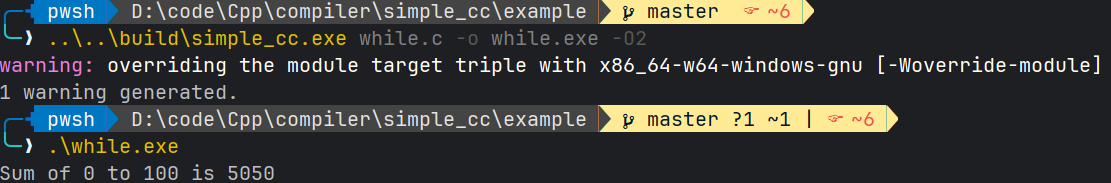
\includegraphics[width=\textwidth]{33.png}
\caption{编译运行结果}
\label{fig:output}
\end{figure}

\section{其他}

\subsection{AI 的使用}
在项目的实现过程中,使用了 AI 辅助编程工具 \texttt{GitHub Copilot},但由于项目的复杂性和规模,AI 仅在部分代码的编写中提供了帮助,主要用于生成函数的注释和部分代码片段。AI 的使用并未影响项目的整体设计和实现,所有核心功能均由本人独立完成。

\end{document}
